\newenvironment{tmpfigure2}
  {\venueifelse{\begin{figure}[t]}{\begin{figure}[b]}}
  {\end{figure}}

\begin{tmpfigure2}
    \neuripsonly{\vspace{-1.5\baselineskip}}
    \centering
    \begin{subfigure}[t]{0.325\textwidth}
        \centering
        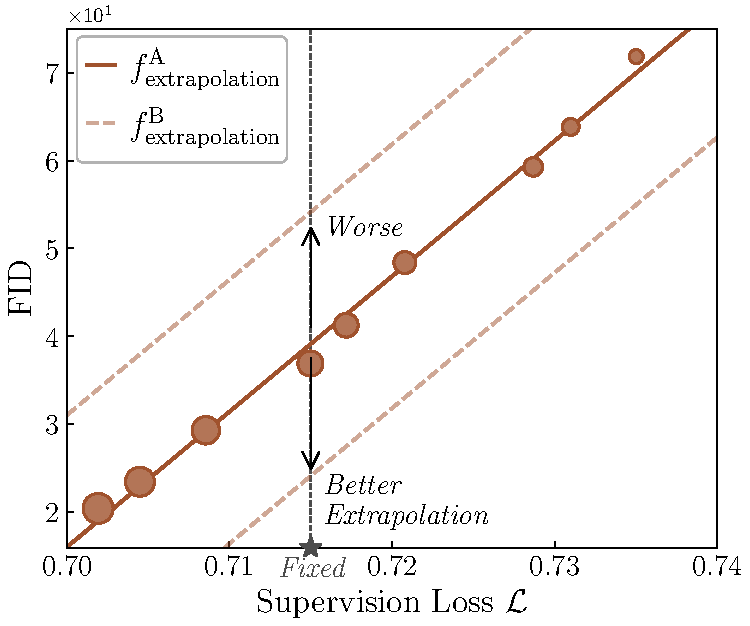
\includegraphics[height=0.86\textwidth]{figures/performance/pat_verification_a}
        % \vskip -0.3\baselineskip
        % \caption{
        % \xsienna{\textbf{Scaling law}}
        % % Supervision loss vs.\ FID, enabling disentanglement of extrapolation from supervision.
        % }
        \phantomcaption
        \label{fig:pat-verification-a}
    \end{subfigure}
    \hfill
    \begin{subfigure}[t]{0.325\textwidth}
        \centering
        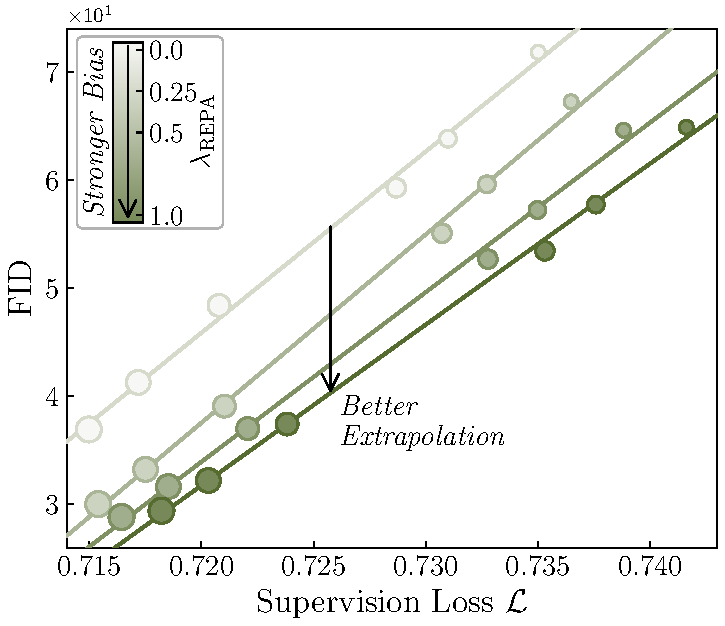
\includegraphics[height=0.86\textwidth]{figures/performance/pat_verification_c}
        % \vskip -0.3\baselineskip
        % \caption{
        % \xolive{\textbf{REPA}}
        % % Varying Alignment strengths $\lamrepa=\{0.0, 0.25, 0.5, 1.0\}$.
        % }
        \phantomcaption
        \label{fig:pat-verification-b}
    \end{subfigure}
    \hfill
    \begin{subfigure}[t]{0.325\textwidth}
        \centering
        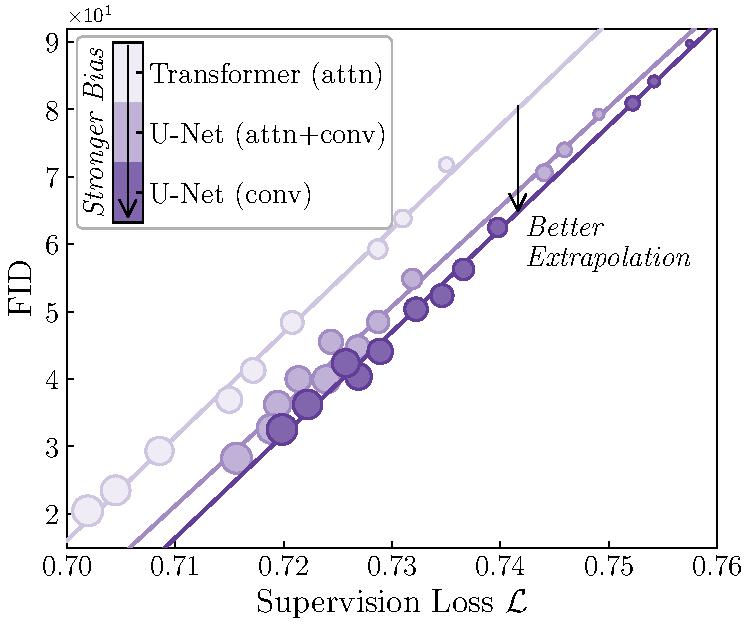
\includegraphics[height=0.86\textwidth]{figures/performance/pat_verification_b}
        % \vskip -0.3\baselineskip
        % \caption{
        % \xxpurple{\textbf{Transformer vs.\ U-Net}}
        % % From Transformer (attn) $\to$ U-Net (attn+conv) $\to$ U-Net (conv).
        % }
        \phantomcaption
        \label{fig:pat-verification-c}
    \end{subfigure}
    \vskip -1.5\baselineskip
    \caption{
    \textbf{Illustration of the decomposed analysis of generative performance.} (a) FID (\emph{$y$-axis}) is plotted as a linear function $f_\text{extrapolation}$ (\xsienna{\emph{line}}) of supervision loss $\Ls$ (\emph{$x$-axis}). $f_\text{extrapolation}$ depends on the training recipe (A vs.\ B) and is more efficient when shifted downward. Our analysis shows that (b) \xolive{REPA} and (c) \xxpurple{U-Net (vs.\ transformers)} yield more efficient $f_\text{extrapolation}$, i.e., \emph{better extrapolation behavior}. Marker size indicates each model’s total training compute (FLOPs).
    }
    \label{fig:pat-verification}
    \vskip -1.75\baselineskip
\end{tmpfigure2}